
\chapter{System Process Diagram}




\section{Sequence Diagram}
ProConf helps to manage the people involved in organizing a conference,track chair or co-chair or member,reviewers and authors, notifying readers and registered participants and assisting with the correspondence.In sequence diagram,at first chair create conference website,author signup page,open or close submission,sent email to the people involved in organizing a conference. Author making a submission when chair open submission,upload a file in one account.Track chair assign reviewer,assign paper,gives comment about this paper after reviews.Chair and Track chair or co-chair show all submitted paper.Reviewer reviews paper,give marks assigned paper.Chair accept or reject paper after reviews and sent  notification,email to author.

\begin{figure}[h!]
\centering
  % Requires \usepackage{graphicx}
  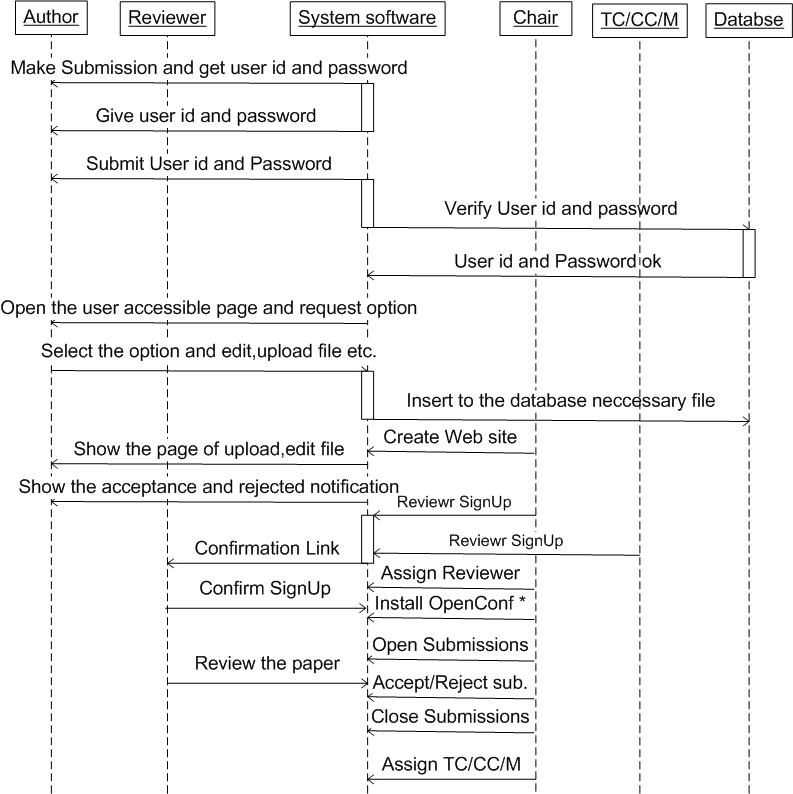
\includegraphics[width=6in,height=3in]{pic/seq1}
   \caption{Sequence Diagram}\label{sequence}
\end{figure}


\section{Activity Diagram}
\subsection{Activity Diagram of Chair’s}
Chair install this system,create conference website,assign reviewer,assign track chair or co-chair or member,accept or reject paper,sent email to the people involved in organizing a conference.

\begin{figure}[h!]
\centering
  % Requires \usepackage{graphicx}
  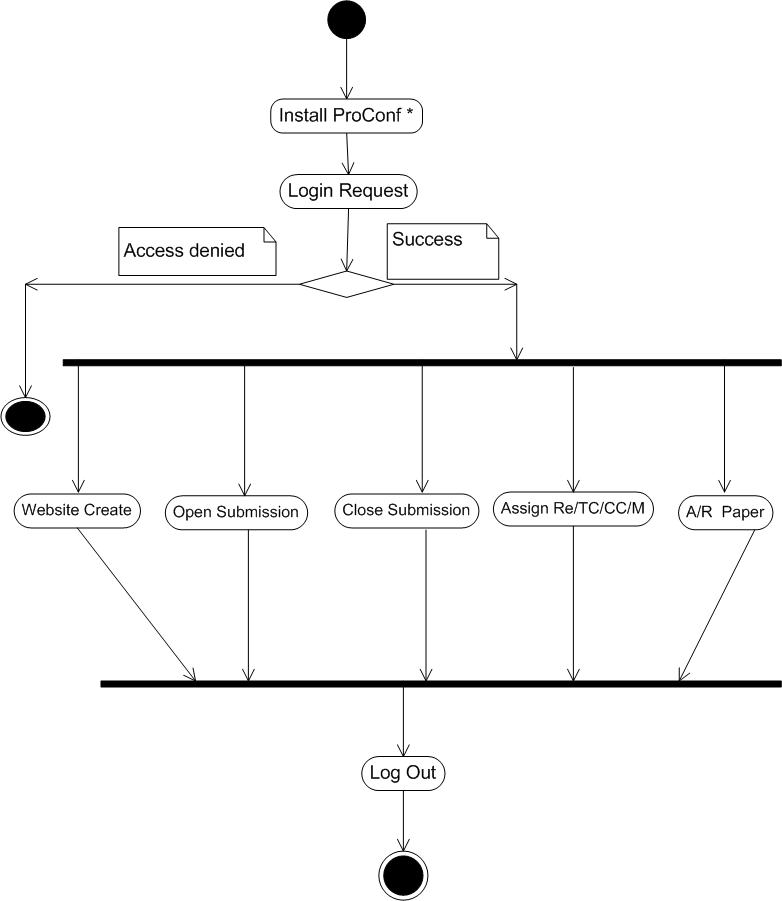
\includegraphics[width=6in,height=6in]{pic/acc}
  \caption{Activity diagram of chair’s}\label{activityc}
\end{figure}
\newpage

\subsection{Activity Diagram of Author’s}
Author making a submission,upload a file,edit file in one account.There will be different color exist to easily identify if file not upload,accept or reject paper,pending paper.
\begin{figure}[h!]
\centering
  % Requires \usepackage{graphicx}
  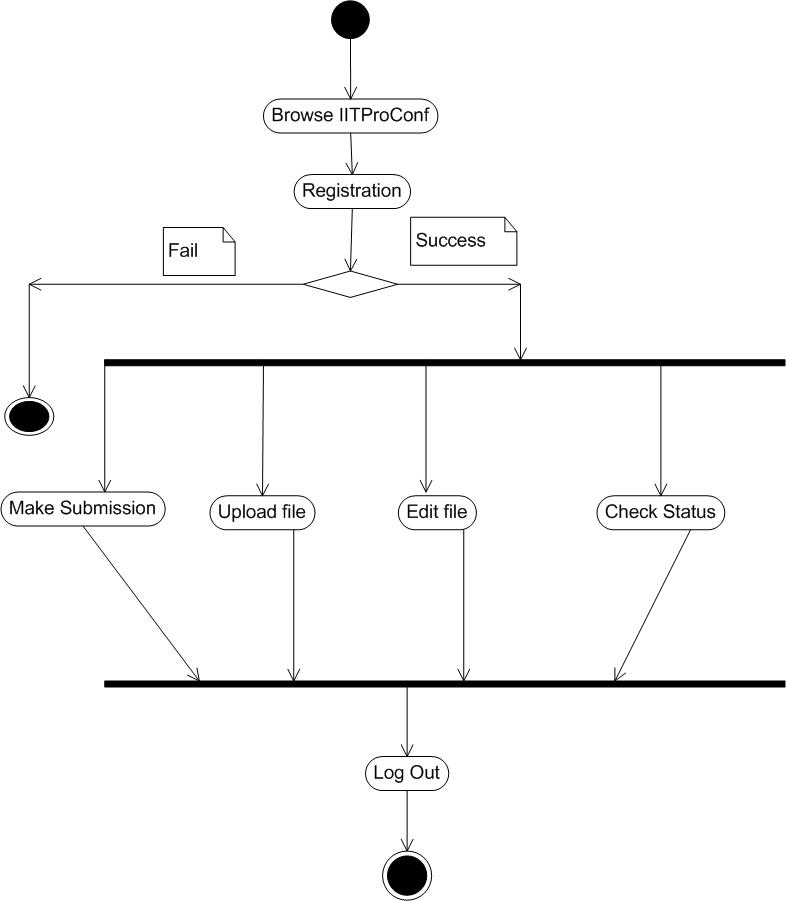
\includegraphics[width=6in,height=7in]{pic/aca}
  \caption{Activity diagram of  author’s}\label{activitya}
\end{figure}

\subsection{Activity Diagram of Track Chair’s or Co-Chair}
Track chair assign reviewer,suggest accept or reject paper,sent email to the people involved in organizing a conference.
\begin{figure}[h!]
\centering
  % Requires \usepackage{graphicx}
  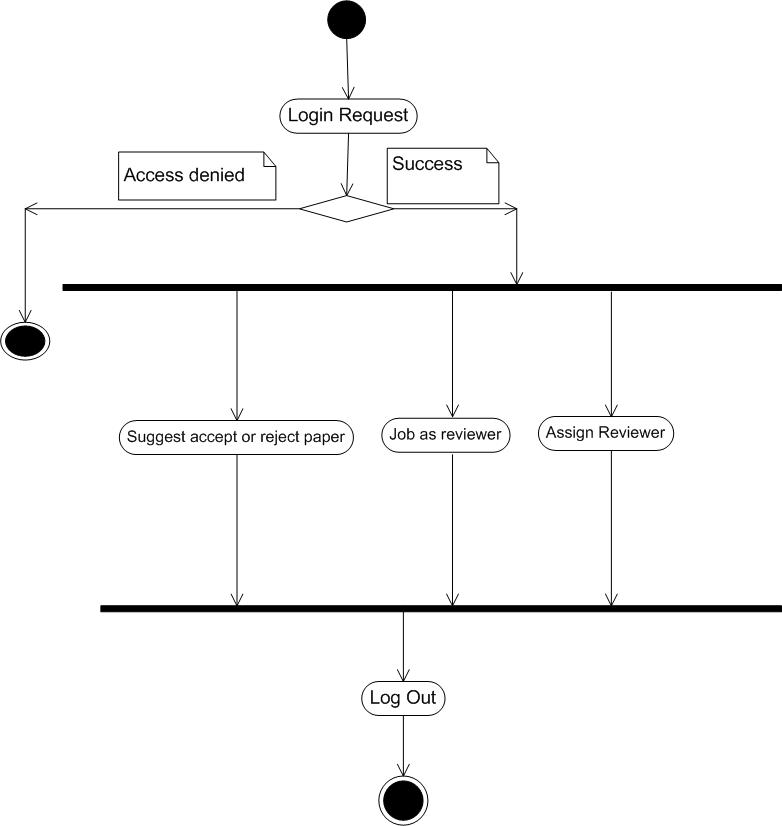
\includegraphics[width=6in,height=7in]{pic/track}
  \caption{Activity diagram of track chair’s or co-chair}\label{activitya}
\end{figure}


\section{Activity Diagram of Reviewer}
Reviewer reviews paper,give marks assigned paper.

\begin{figure}[h!]
\centering
  % Requires \usepackage{graphicx}
  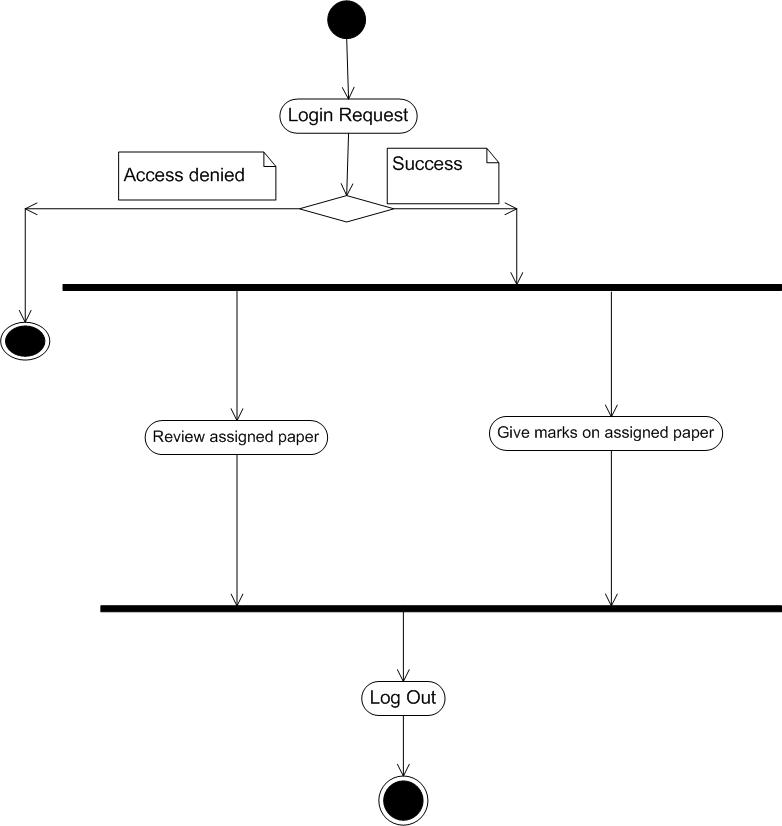
\includegraphics[width=6in,height=7in]{pic/reviewdiagram}
   \caption{Activity Diagram of Reviewer}\label{activityr}
\end{figure}









